%% This is the Project Description For IHCI group Project
%%
%% Group Members:
%%% Shivoy Arora
%%% Tushar Kumar
%%% Gaurav Gupta
%%% Ayush
%%% Manish
%%% Ankit Kumar Pal

\documentclass[acmtog]{acmart}
% \documentclass[manuscript,screen,review]{acmart}

\AtBeginDocument{%
  \providecommand\BibTeX{{%
    \normalfont B\kern-0.5em{\scshape i\kern-0.25em b}\kern-0.8em\TeX}}}

% Remove copyright
\setcopyright{none}

\usepackage[utf8]{inputenc}

\begin{document}

\title{HELP DESK-solve your issues}

%%% Authors
\author{Shivoy Arora (2021420)}
\email{shivoy21420@iiitd.ac.in}

\author{Tushar Kumar (2021212)}
\email{tushar21212@iiitd.ac.in}

\author{Gaurav Gupta (2021148)}
\email{gaurav21148@iiitd.ac.in}

\author{Ayush (2020501)}
\email{ayush20501@iiitd.ac.in}

\author{Manish (2021164)}
\email{manish21164@iiitd.ac.in}

\author{Ankit Kumar Pal (2021132)}
\email{ankit21132@iiitd.ac.in}

\date{March 2022}

\begin{abstract}
    In their day-to-day life, people face a lot of difficulties like poor infrastructure, low maintenance of their area, and other social issues. These are the problems that need political support and assistance. But in most cases, these issues remain unsolved or take a long time to resolve. The main reason behind this is the poor communication between the political leaders and people. Most of the time people fail to judge who then have to seek help or in which government department they should go for their issue. Here we come up with a solution to this problem. Our program plays a key role to create a bridge between the political representatives and people. We are providing a platform to register their issues and complaint. They will get the contact details of the concerned political leader who can solve their issue. The program will also tell them about the government office where they should visit. Their complaint will also go to their concerned leaders. Leaders will have a profile in our programs that shows how they deal with the complaints. All our program will do is that helping people to hold the government accountable and efficient. This will create awareness about all the rights of people. Also here we are providing an assistant by providing steps to apply for some of the basic documents like VOTER ID CARD, AADHAAR CARD, etc.
\end{abstract}

\maketitle

\section*{Introduction}
One of our group members told us how a small issue of road repair in their locality takes up more than three months and a lot of efforts they have made. That story looks relatable to all of us as once in our life we have tried to solve any social issue and it took much more time as thought and takes too much effort. Most of us when trying to solve any problem don’t know about the procedure. We don’t know who we have to meet to seek help for the issue. There is no direct method by which we can communicate to our political representative about the issue. Soling issue through government officials is too long because of poor communication between people and officials. Many times when we tried to file an issue on any government website, we fails to find the correct website and procedure. Although we can improve the functioning of government websites but finding the correct path will reduce the solution time. That whole scenario put us thinking about how we can do something to improve this. Although there are some solutions available like complaint boxes/registers in government offices they are hard to get. We have planned to make a program that will improve communication and problem solving will be much easier. The program allows user to enter their issues along with their location, our program will provide the necessary detail of the political representative of that area who can solve the issue. The program will also provide some links to useful government websites where they can file the issue. The steps of doing so are also provided. Anyone who is active in solving the daily issues can use our program. All political leaders are also the stakeholders of the program as they can look after the complaints raised in their jurisdiction. The media also can use our program to allow the public to know about the working efficiency of any political leader. We have faced some of the challenges like getting correct information about the leaders is very difficult, constantly updating in government staff also poses a problem. We are dealing with these and try to give the best we can.

\section*{Methodology:}
% Problem Definition
\section{PROBLEM DEFINITION AND IDENTIFYING STAKEHOLDERS}

%% Define the problem
\subsection{Define the problem}
We face a lot of issues in our daily life. Some of them are personal while some are social. Social issues need some kind of political involvement and administrative assistance from the government side. But in our daily life, there is no such place or way by which we can directly approach our political representatives. Maybe some sort of solution is available but it is not within the reach of the common man. There is no transparency between people and political leaders. Most of the people don’t know about their political representative and their approach to solving an issue. We find it a very important issue we are dealing with today.

%% Background of the problem and motivation
\subsection{Background of the Problem and Motivation}
One of our project group members, who live in a semi-remote area told us about the problem of bad road conditions in his area. Due to this, there were no means of transport and accidents had turned very common for them. One day some people of the society gathered to complain against it as it was making their normal life difficult. So they decided to meet their MLA to report about the bad road conditions. The MLA listened to them and asked to go to the Municipality Office, as they are responsible for this. Then they visited the Municipality Office where they didn’t get proper assistance. It took more than three months and a lot of effort to get the work done. After listening to him we thought to design something that will “Repair the road between the people and the government”.

%% Stakeholders
\subsection{Stakeholders and their role}
\subsubsection{Common People}
As in politics, common people play a significant role. Various issues are faced by people which need political support get resolve
\subsubsection{Political representatives}
Political leaders (i.e. MPs, MLAs, and counsellors) are at the center of this issue as they are the only ones who can resolve the issue raised
\subsubsection{Government officials}
Any order or solution of an issue given by a political representative is implemented by government officials
\subsubsection{Media}
The role of media is to check the accountability and issue-resolving strategy of the government.

%% Other products
\subsection{What other products exist which are trying to solve similar problems?}
\begin{enumerate}
    \item Complain register/box available at the residence of political leaders and government offices.
    \item Government websites of different departments.
    \item Government dictionary for all govt. websites: - \url{https://igod.gov.in/}
    \item Publishing an issue in media that makes it more famous. 
\end{enumerate}

%% Limitations of other products
\subsection{Limitation of current products}
Complain registers are sometimes missing or hard to get from the corresponding official. It is time-consuming. In some places, such complaint systems don’t have any value.
Government websites need some previous knowledge to deal with them. These are very slow due to low maintenance.
Government dictionaries are too much hard to be handle as they have thousands of websites. It causes a cognitive load on the user while using them.
Publishing any issue in media is a long process and it takes more than the desired time to get resolved.

%% How novel is our solution
\subsection{How could/would your solution be novel?}
In our design we will provide the following facilities which make the process easier:
\begin{enumerate}
    \item User will enter their issue and their location. Our program will find the authorized political leader or govt. official available at that time to solve that issue.
    \item Our program also provides the link to a suitable website if they want the solution to be online.
    \item A notification has been sent to the concerned political leader or govt. official about the issue which has been raised in their area.
    \item There is a profile system for every political representative (describing the no. of issues solved by them) so that users can find the accountability and efficiency of a representative.
    \item  User will get notified about the latest policies made by the government.
    \item Program will provide assistance to users while applying for some important documents (such as VOTER ID CARD, AADHAAR CARD, DRIVING LICENSE, etc.) 
    \item Our program have some stuff available that help user to understand the political structure and function of the country.
    \item Our program will make the user aware of their rights as stated by the government.
\end{enumerate}

%% Challenges we will face
\subsection{Challenges we will face}
\begin{itemize}
    \item There is no correct contact information available about all the political leaders.
    \item Leaders and government officials keep changing and there is no place where all these updates are available
    \item Many of government websites don’t give us access.
\end{itemize}

%% Requirement gathering
\section{REQUIREMENT GATHERING}

\begin{description}
    %%% Google Form
    \item[(A)] We have tried to reach the audience by the means of a google from which contained some questions related to the issue we are solving. We have got the following analysis

    \begin{figure}[H]
        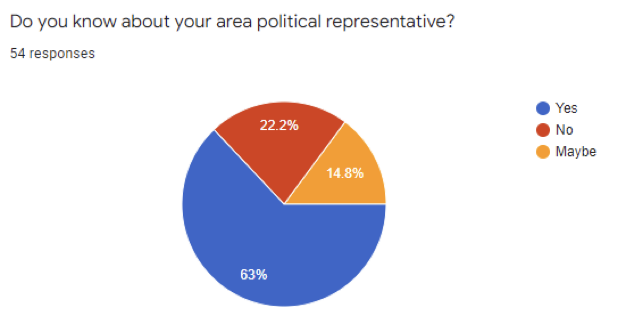
\includegraphics[width=8cm]{Resources/q1}
        \caption{Question 1}
        \label{fig:q1}
        \Description{Do you know about your area's political representative}
    \end{figure}

    In this question, we ask people whether they are familiar with (or know) their regional politics. According to the responses we come to know that majority of people are known to their political representative. But there is a group of people (approx. 37\%) who don’t know about their political leader. Our task is to make all people aware of their political representative.

    \begin{figure}[H]
        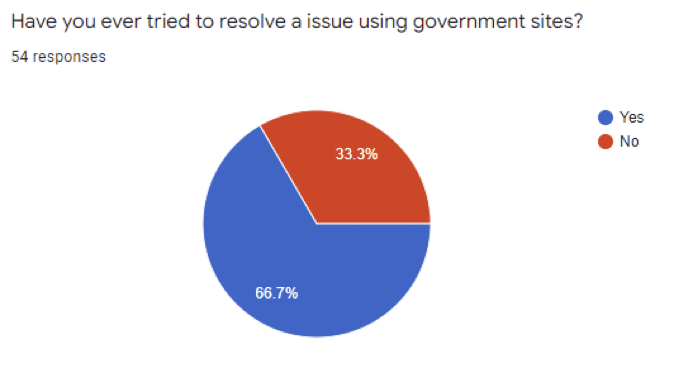
\includegraphics[width=8cm]{Resources/q2}
        \caption{Question 2}
        \label{fig:q2}
        \Description{Have you ever tries to resolve a issue using government sites}
    \end{figure}

    From the above data we analyse that majority of people are engaged somehow in solving any issue either social or personal which need the interference of political leaders.

    \begin{figure}[H]
        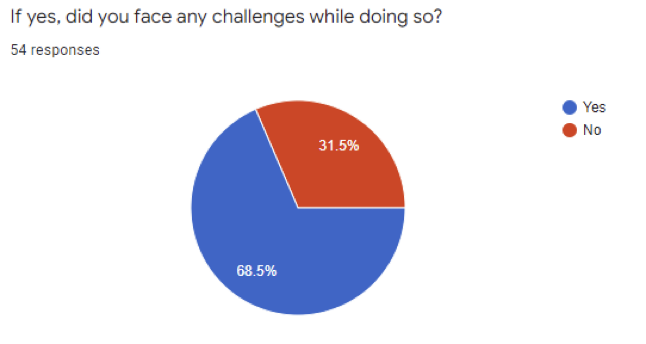
\includegraphics[width=8cm]{Resources/q3}
        \caption{Question 3}
        \label{fig:q3}
        \Description{If yes, did you face any challenges while doing it}
    \end{figure}

    The above data clearly states that the peoples who are engaged in solving any issue, a huge majority of people face challenges while resolving it. This is our main aim to make this process of solving issues simpler so people don’t face too many challenges.


    \begin{figure}[H]
        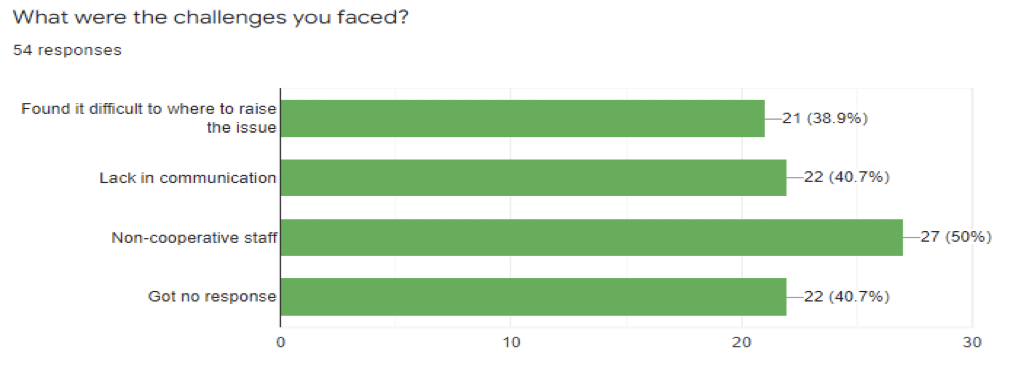
\includegraphics[width=8cm]{Resources/q4}
        \caption{Question 4}
        \label{fig:q4}
        \Description{What were the challenges you faced}
    \end{figure}

    In continuation of the above ques, we give some general challenges which were faced. Most people face all of the provided issues. But the issue of non-cooperative staff is faced by most of them. This challenge arises because of corruption in our system and there is no cross-checking and transparency. People not getting any response regarding their issue is also because of the same reason.

    \begin{figure}[H]
        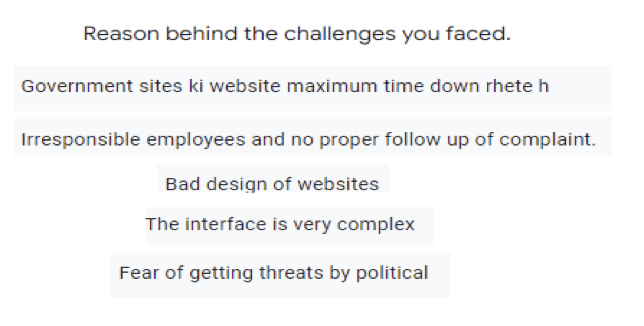
\includegraphics[width=8cm]{Resources/q5}
        \caption{Question 5}
        \label{fig:q5}
        \Description{Reasons behind the challenges faced}
    \end{figure}

    Here are some other reasons for the challenges faced by the people while solving an issue. We analyse that most people face problems while using a government website. This is because of the bad design and complex interface of websites. 

    \begin{figure}[H]
        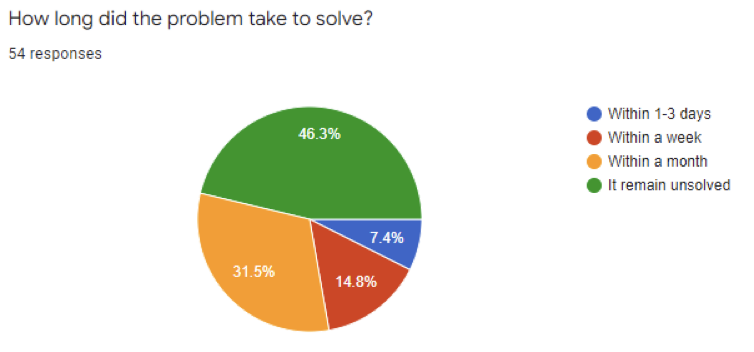
\includegraphics[width=8cm]{Resources/q6}
        \caption{Question 6}
        \label{fig:q6}
        \Description{How long did the problem take to solve}
    \end{figure}

    We ask the audience to respond to the ques about the time which it takes to resolve an issue. Approx. half of them responded that their issue remains unsolved or it may take up to a month to solve the issue.

    \begin{figure}[H]
        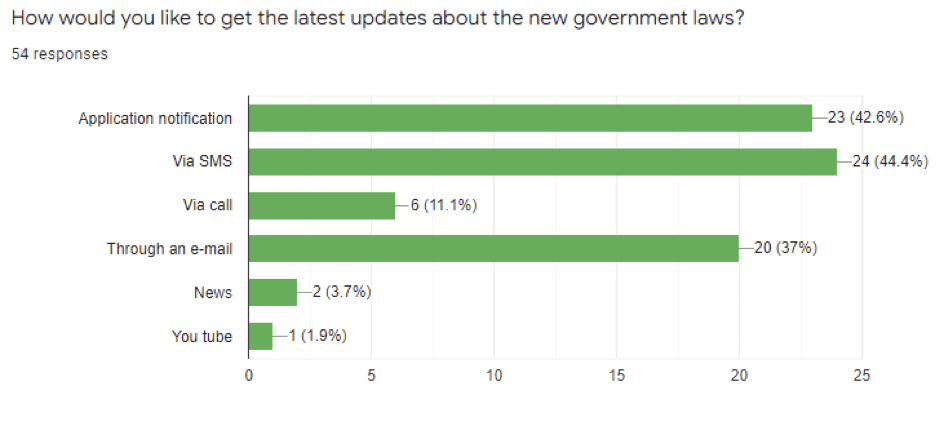
\includegraphics[width=8cm]{Resources/q7}
        \caption{Question 7}
        \label{fig:q7}
        \Description{How would you like to get the latest updates about the new government laws}
    \end{figure}

    The above poll shows that most people are interested to get an update on all the policies and decisions made by the government. Most of them wanted to get notified through SMS on their phone or by the application notification of our program. Those who spend their time on PCs and laptops want to get notified through E-mail.

    \begin{figure}[H]
        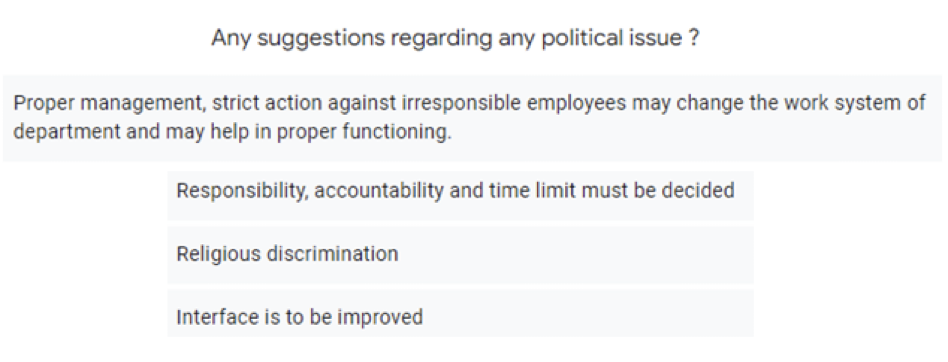
\includegraphics[width=8cm]{Resources/q8}
        \caption{Question 8}
        \label{fig:q8}
        \Description{Suggestions}
    \end{figure}

    Here are some other suggestions related to our program. We will take up these suggestions very strongly while designing our program

    %%% References
    \item[(B)] We tried to study some documents and data available on the internet.
    
    \begin{enumerate}
        \item It is one of the major problems of the rural side of our country, "Electricity Supply". Many governments have made and demolished over the years, but this problem still stands tall against the people living in those rural areas. Even some people for the rural areas of Uttar Pradesh reported that only when the bill arrives, do we know there's power, and when a crow dies and falls off the electric pole, we know there is some current in the wire because electricity doesn't come to their homes. When asked why they don't complain against this, they answered we don't know where to complain. They added that no one there is educated enough and has no idea about the processes.
        \footnote[1]{\url{https://www.hindustantimes.com/india-news/the-challenges-of-india-s-grand-rural-electrification-scheme/story-pLilYKEh7At99BoSeERqXM.html}}
        \item Indian government is very actively working towards e-governance and the citizens with access to internet-enabled computers and smartphones too look forward to an easier life. After all, who doesn’t like to use the online option provided by almost all the organizations and save time by avoiding the long queues at different utilities and departments. However, the biggest irony is that many governments or PSU websites that offer an online solution for the public or enterprises are more of an online headache for them. Some of these have navigational issues, others are updated only once in a few months, while many others have serious design or usability flaws.
        \footnote[2]{\url{https://timesofindia.indiatimes.com/computing/8-worst-indian-government-websites/articleshow/14303498.cms}}
        \item The Digital India initiative may be aiming to make all government services electronically available, but a recent study has found 10 government websites in Delhi lacking several transparency parameters. The study, published in Delhi Citizen’s Handbook 2016, audited the websites against predefined parameters of Section 4 of the Right to Information (RTI) Act that sets guidelines for proactive disclosure of information by government agencies without the public having filed RTI queries. Nine out of the 10 websites could not even meet 60\% of the compliance points, said the study, conducted by the Centre for Civil Society.	
        \footnote[3]{\url{https://economictimes.indiatimes.com/news/politics-and-nation/digital-india-government-websites-fail-to-clear-transparency-test/articleshow/53781991.cms?from=mdr
        }}
        \item Ambala, a beautiful town in Haryana, famous for many tourist attractions like Bhawani Amba Temple, Badshahi Bagh Gurudwara, and large Indian Army base and Indian Air Force presence within its cantonment area. but still being beautiful town citizens of Ambala who are living in somewhere in the local areas like (novelty chowk) are facing issues in living their life and the major problem is they are going through is the harsh condition of roads. Which causes difficulty in the daily movement of people. After asking from them we came to know that many of them don’t even know where they have to complain about the road related concern. Some of them said that very few people show interest in this concern. We came to know from that they some people complain much time but didn’t get any responses from the authorities, and also no action and progress are shown till now. 
        \footnote[4]{\url{https://youtu.be/ON9o-lYcq14}}
    \end{enumerate}

\end{description}


% ANALYSIS AND FUTURE WORK
\section*{Analysis and future work}
In the process of designing this program, we analyse the data gathered from the audience, study some news articles and evaluate some government websites. We found the common problem which the people are dealing with-“They don’t know the procedure of raising an issue”.

\noindent Most of the time people get distracted to some other path when they try to solve any problem.

\noindent Our program will keep them on the right path and reduces stress. Our future work will cover the IDEATION, LOW FI PROTOTYPING, HI-FI PROTOTYPING, and EVALUATION of the program. We will keep looking forward to making the program better.

% CONCLUSION
\section*{Conclusion}
We have tried to collect a sufficient amount of data from the audience and the internet related to our project. We have circulated some questionnaires, study some news articles, and evaluated the present solutions. We find that all of them have similarities in solving an issue. They don’t allow any direct interaction between officials and people. Many times the websites or other available programs are unable to understand the issue effectively which may lead to a long process and sometimes an unsuitable solution. We have kept all these points in mind while designing our program.

% CONTRIBUTION
\section*{Contributions}
\begin{enumerate}
    \item Shivoy Arora (2021420):
    \begin{itemize}
        \item Ideation
        \item Overleaf
        \item Resources gathering
        \item Analysis and future work
    \end{itemize}

    \item Tushar Kumar (2021212):
    \begin{itemize}
        \item Ideation
        \item Introduction
        \item Methodology
        \item Resources gathering
    \end{itemize}

    \item Gaurav Gupta (2021148):
    \begin{itemize}
        \item Ideation
        \item Methodology
        \item Resources gathering
        \item Conclusion
    \end{itemize}

    \item Ayush (2020501):
    \begin{itemize}
        \item Ideation
        \item Introduction
        \item Methodology
        \item Resources gathering
    \end{itemize}

    \item Manish (2021164):
    \begin{itemize}
        \item Ideation
        \item Methodology
        \item Resources gathering
        \item Analysis and future work
    \end{itemize}

    \item Ankit Kumar Pal (2021132):
    \begin{itemize}
        \item Ideation
        \item Abstract
        \item Methodology
        \item Resources gathering
        \item Conclusion
    \end{itemize}
\end{enumerate}



\end{document}
